\section{Rawls: Difference Principle}
\label{equity-sec:diff-prin}

Still developing the distinction between equality and equity, I present the difference principle stated by \citeonline{rawls:1971}. Rawls was a \gls{USA} citizen and political philosopher in the liberal tradition \cite{wenar:2021}. His theory structures a society under the lens of an egalitarian economic system.

Hans Traxler\footnote{It is known that Hans Traxler, a Czech illustrator, created the original cartoon in 1976 \cite{traxler:2019}. But it is unknown the artist who translated it for English version. See more details \url{https://historyof.place/the-politics-of-disability-from-6th-century-china-to-the-industrial-revolution/}.} created an excellent illustration (Figure \ref{fig:fair-selection-traxler}) that helps us to delve into this discussion. In the first moment, it is natural to assume that equal treatment is a synonym for justice. But there are several scenarios, like that presented by Traxler, evidencing the issues that can emerge for our students from this premise. 

\begin{figure}[ht!]
\centering

\caption{\textmd{Illustration translated from original cartoon created by Hans Traxler.}}
\label{fig:fair-selection-traxler}
\fcolorbox{gray}{white}{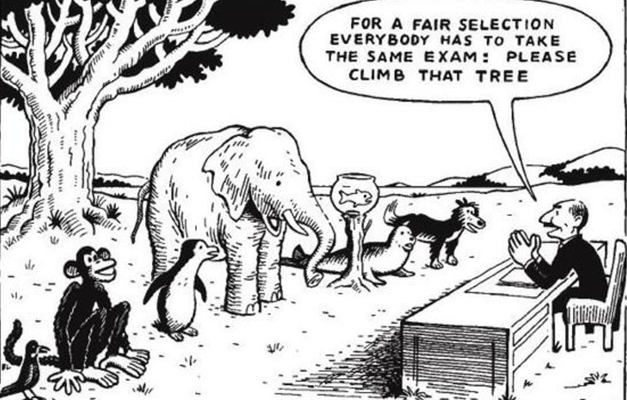
\includegraphics[width=0.8\textwidth]{images/chapter-03/traxler-illustration.jpg}}

\par\medskip\ABNTEXfontereduzida\selectfont\textbf{Source:} Created by Traxler \cite{traxler:2019}.%\citeauthor{manualufpe2020} (\citeyear{manualufpe2020}) \par\medskip
\end{figure}

The crucial point here is that, probably, the underlying reason to apply equal treatment to foster social justice is our seeking equality of opportunities. Equal treatment used to be the default solution to tackle common justice problems in our day-to-day life. But equal treatment is not what we are searching for. We use equal treatment aiming for equality of opportunities. In this way, it will be necessary to discern when to make use of equal treatment or not. Just in this point Rawls' principle plays an essential role in the discussion about equality and equity.

Rawls' starting point is what he called the “original position” for all people of an imaginary society that does not exist yet. \citeauthoronline{rawls:1971} (\citeyear{rawls:1971}, p.~12) develops this idea clearly, asserting that:
\begin{citacao}
    “[N]o one knows his place in society, his class position or social status, nor does anyone know his fortune in the distribution of natural assets and abilities, his intelligence, strength, and the like. I shall even assume that the parties do not know their conceptions of the good or their special psychological propensities. The principles of justice are chosen behind a veil of ignorance”.    
\end{citacao}

And what are these principles? \citeauthoronline{rawls:1971} (\citeyear{rawls:1971}, p.~83) lists two ones that would naturally arise from the veil of ignorance. The second principle states the following:
\begin{citacao}
    “2. Social and economic inequalities are to be arranged so that they are both:
    
    \hspace{0.5cm} (a) to the greatest benefit of the least advantaged, consistent with the just savings principle, and
    
    \hspace{0.5cm} (b) attached to offices and positions open to all under conditions of fair equality of opportunity".
\end{citacao}
 
Part (a) of this principle is what Rawls named the difference principle. The difference principle is a rational justification for a differentiated treatment aiming to promote equality of opportunities.

Why more boxes for the child (Figure \ref{fig:equality-vs-equity})? Because we want to promote equality of opportunities. Thus, we guarantee the greatest benefit to the least advantaged originally. Why can we not apply the same exam for all (Figura \ref{fig:fair-selection-traxler})? Because we would not guarantee equality of opportunities for everybody. It is possible to connect this to what \citeauthoronline{parker:2015} (\citeyear{parker:2015}, p.~4) assert about the difference principle:
\begin{citacao}
    “[Strict] equality is privilege agnostic and implies giving every student equal opportunities no matter where they start. Justice is privilege sensitive and involves giving some students more opportunities than others based on how disadvantaged the student might be”.
\end{citacao}
Fostering privilege sensitivity matters if we want to build a school environment that does not reproduce the pre-existing inequalities in our society. Restructuring the school in an equitable direction signals an achievable changing perspective for society in seeking a fairer world.

Although the difference principle occupies a prominent position concerning equity discussion, the whole Rawls' theory of justice doesn't have the same acknowledgment. Many researchers (like me) are not interested in establishing a foundational theory (bearing in mind that Rawls' original position is only relevant to establishing a public reason in a collective debate). The reality is that it is not possible to reinitialize the whole society from this justice perspective. One more interesting proposal can be to identify and highlight the main aspects to consider to discuss equity appropriately (including by using the difference principle). \citeonline[p.~94]{robeyns:2005} presents the \glsfirst{CA} as a possibility to address these questions in a framework perspective:
\begin{citacao}
    “Note that the capability approach is not a theory can explain poverty, inequality or well-being; instead, it rather provides a tool and a framework within which to conceptualize and evaluate these phenomena. Applying the capability approach to issues of policy and social change will therefore often require the addition of explanatory theories”.
\end{citacao}
Thus, I will present \gls{CA} in the next section from the perspective of an equity 
 conceptual framework.
        
